\documentclass[10pt]{article}
\usepackage{tmlr}
\usepackage{amsmath,amssymb}
\usepackage{booktabs}
\usepackage{graphicx}
\usepackage{hyperref}
\usepackage{url}

\title{Leaderboard Overfitting on Kaggle, Revisited:\\ A Pre-Specified Re-Test and the Limits of Aggregate Scores}

\author{\name Anonymous authors \\ \addr Paper under double-blind review}

\def\month{MM}
\def\year{YYYY}
\def\openreview{\url{https://openreview.net/forum?id=XXXX}}

\begin{document}
\maketitle

\begin{abstract}
\citet{roelofs2019meta} compared public and private leaderboard scores in 120 Kaggle competitions and found little evidence of substantial adaptive overfitting. We re-test that conclusion on competitions that ended after their sample, with the analysis plan fixed and publicly archived before any new score was read. We first reconstruct the original study from Meta Kaggle. All 120 competitions are recovered and the five accuracy outliers reproduce, but the published test-set sizes are incompatible with the recorded scores for 11 of 32 accuracy competitions. On 487 later competitions, the median public--private gap of accuracy and AUC competitions differs from the original sample by less than the thresholds we set in advance. We also report a within-team quantity the original design did not examine: in 68\% of later competitions, and 68\% of the original ones, teams' later submissions favour the public leaderboard more than their earlier ones, by about one percent of the distance between a median and a top-decile team. This divergence is what adaptation to public feedback would produce, and under a random public--private split it could not arise without some dependence on that feedback. For most competitions the split cannot be verified, and we show that a model-dependent difference between the two sets can produce the same pattern. We therefore report the divergence as consistent with adaptation, not as a measurement of it, and set out what aggregate leaderboard scores can and cannot identify: adaptation, test-set sizes, and selection effects among top submissions.\footnote{A large language model assistant was used to design and implement the analyses and to draft text, under the authors' direction. The authors reviewed all content and are responsible for it.}
\end{abstract}

\section{Introduction}

A Kaggle competition gives every submission two scores. The public score is computed on one part of the test set and shown at once; the private score is computed on the rest and revealed when the competition ends. The public part is a test set reused thousands of times, the private part is used once, and the difference between them is a natural experiment on adaptive overfitting \citep{dwork2015reusable,blum2015ladder}. \citet{roelofs2019meta} used this design on 120 competitions and concluded that overfitting ``did not pose a significant danger''. Together with test-set replication studies \citep{recht2019imagenet,yadav2019cold}, the result underpins the view that benchmark reuse has been less harmful than theory allows, and it is still cited in that role \citep{sculley2025position}.

The sample behind the result ends in April 2019. Since then the platform has added competitions in which code is re-run on hidden data, a monthly series on synthetic data, and metrics defined per competition. Later descriptive work reports noticeable public--private discrepancies \citep{bonisch2025chronicles,burtch2026monoculture}, though with measures that select each team's best public submission or that are not accompanied by tests. Our searches on 15 and 16 November 2026 found no peer-reviewed re-test of the 2019 result on later competitions; this is a statement about those searches, not proof of absence.

This paper makes four contributions.
\begin{itemize}
\item An independent reconstruction of the 2019 study from the public data, with every discrepancy documented (Section~\ref{sec:recon}).
\item Minimum compatible test-set sizes computed from accuracy scores, graded by how far independent evidence supports them. In our reconstruction they allow the original null-model test to be computed for 33 of the 34 original accuracy competitions, where the published sizes allow 19.
\item A re-test on 487 later competitions with four pre-specified confirmatory tests (Section~\ref{sec:confirm}), followed by secondary and exploratory analyses that are labelled as such.
\item A within-team temporal divergence between public and private scores, together with an account of the assumptions under which it would indicate adaptation and a demonstration that those assumptions matter (Sections~\ref{sec:methods} and~\ref{sec:explore}).
\end{itemize}

\section{Related work}

\paragraph{Adaptive data analysis.} Reusing a holdout set can invalidate its estimates \citep{dwork2015reusable}, and leaderboard mechanisms have been designed to limit this \citep{blum2015ladder}. Theory also predicts when reuse should be benign: similarity between models reduces the effective number of queries \citep{mania2019similarity}, and problems with more classes are harder to overfit by reuse \citep{feldman2019multiclass}.

\paragraph{Empirical studies of reuse.} New test sets for ImageNet and MNIST showed accuracy drops but stable rankings \citep{recht2019imagenet,yadav2019cold}. \citet{roelofs2019meta} is the largest study of reuse within competitions. Its authors listed open questions that motivate our secondary analyses: regression competitions, uncertainty for metrics other than accuracy, and a suggested minimum of 10,000 test examples.

\paragraph{Later analyses of Kaggle.} \citet{bonisch2025chronicles} report normalised public--private discrepancies across competitions, without formal tests. \citet{burtch2026monoculture} reconstructs leaderboards for 158 contests to relate code convergence to the public--private shift of each team's best public submission, and notes that this quantity is biased by selection. Neither re-tests the 2019 analysis.

\section{Reconstructing the original study}
\label{sec:recon}

\paragraph{Sample.} The 120 competition identifiers are listed in the original appendix. All are present in the Meta Kaggle snapshot of 15 November 2026 \citep{metakaggle}. We recover 1,510,406 pre-deadline submissions with both scores, against 1,513,918 published; 46 of the 120 counts match exactly and none differs by more than 2.6\%. The latest deadline in the sample is 4 April 2019, and the next competition that meets the published inclusion rule, with a deadline of 9 April, is absent. We do not know the date of the original extraction. As a cohort convention inferred from the included sample, we start our extension after 4 April 2019.

\paragraph{Inclusion rule.} The published rule is at least 1,000 pre-deadline submissions and one of five metrics. Applied to the current data it yields 28 further competitions inside the original window. Of these, 26 report a public share of 0 or 100 percent, which suggests an unstated requirement that a real split exists.

\paragraph{Headline pattern.} The five largest mean accuracy gaps belong to the five competitions the original paper names as outliers.

\paragraph{Test-set sizes.} Unweighted accuracy times the number of scored examples must be a whole number. For 11 of the 32 accuracy competitions with published sizes, the published sizes fail this check. The clearest case is the Allstate competition. The paper lists 59,657 public and 139,199 private examples, which sum to the 198,856 rows of the test file; the task scores one prediction per customer, and the file contains 55,716 customers. The original text attributes this competition's small $p$-values to its ``198,856 examples''. With customer counts of 16,714 and 39,002, which are the sizes implied by the scores together with the customer total, 1.3\% of submissions have $p \le 0.05$ under the original null model; a normal approximation with the published counts gives 74.6\%. We make no claim about what the original code computed. In the other ten cases the smallest sizes compatible with the scores are: off by one from the published sizes, or with public and private exchanged (four cases); the same total with a different split (three); far smaller than published (two); and identical for both sets, in a competition where every submission has identical public and private scores (one). Only the Allstate total is confirmed by an independent source.

\paragraph{Unspecified choices.} Submission dates have day precision, so the first submission of a team is not always identifiable; the handling of ties at the top-10\% cutoff is not stated; and the tail probability is inclusive in the main text and strict in the appendix. We use submission identifiers to order submissions within a day, keep all ties, and use the inclusive tail.

\section{Methods}
\label{sec:methods}

\paragraph{Cohorts.} $O$ is the original sample. $E$ contains competitions with a deadline after 4 April 2019 and no later than 15 November 2026. $W$ contains earlier regression competitions, which the original study excluded by design. A competition is analysed if it has at least 1,000 pre-deadline submissions, reports a public share between 1 and 99 percent, has at least 1,000 scored submissions from non-benchmark teams, and does not have identical public and private scores for at least 99\% of submissions. This leaves 114 competitions in $O$, 487 in $E$ and 51 in $W$.

\paragraph{Score handling.} Accuracy, AUC and MAP@K are analysed as recorded. For every other metric, both scores are clipped to the 1st--99th percentile range of the competition's public scores, to stop sentinel values dominating means. The bounds come from public scores only, so the treatment is not symmetric in the two sets; Section~\ref{sec:explore} reports results without it.

\paragraph{Gap.} The gap of a submission is its public score minus its private score, signed so that a positive value favours the public score. The mean gap of a competition is the average over its submissions, as in the original study.

\paragraph{Team spread.} To compare metrics we divide by the team spread: the distance between the median team and the top-decile team, measured on teams' median public scores. A relative gap or drift of 0.01 is one percent of what separates a median team from a top-decile team.

\paragraph{Within-team drift.} For each team with at least four submissions, ordered in time, drift is the mean gap of the later half of its submissions minus the mean gap of the earlier half. The drift of a competition is the average over teams. The analysis does not choose submissions by score, and a gap that is the same for every model cancels within each team. A team that tunes to public feedback carries the public noise it has selected into later submissions, which produces positive drift.

Positive drift is not specific to adaptation. If the public and private sets are exchangeable, as under a random split, and submissions do not depend on public feedback, drift has no preferred sign. If the two sets differ in composition, a gap that depends on the model can grow as teams improve, with no use of feedback at all. Drift therefore tests the joint hypothesis of exchangeable sets and feedback-independent submissions. Feedback dependence also includes stopping after a favourable public score, which is not the same as tuning a model.

\paragraph{Minimum compatible sizes and formal test.} For accuracy competitions we compute, separately for public and private scores, the smallest integer on which every score is a whole count. The true number of scored examples is a multiple of it. We grade the result by independent support: (A) the total is confirmed by the test file (Allstate); (B) it equals the published size (21 original competitions); (C) its public share is within one point of the public share reported by the platform, which supports the ratio but not the multiplier (99 competitions); (D) no support (7). Wherever a published size is compatible with the scores it equals the minimum (21 of 21), never a proper multiple. With these sizes we compute, for each submission, the exact two-sided inclusive tail probability of its accuracy difference when its correct answers are split at random \citep{roelofs2019meta}. Results for tiers C and D are conditional on the minimum being the true size.

\paragraph{Independent-resplitting reference for the top decile.} The top 10\% of submissions by public score have a positive expected gap even without adaptation. As a reference we simulate the null model with each submission split independently, select the top 10\% on simulated public scores, and subtract the resulting expected gap from the observed one. Real submissions share one split and are correlated, which changes the gap that selection can produce; for identical submissions it is zero. The reference is a benchmark under independence, not an estimate of the selection effect.

\paragraph{Checks of the computations.} Our exact tail probabilities agree with an independently written implementation on 68,552 submissions to within $10^{-14}$. In a simulation in which teams accept changes that raise their public score, drift is positive whether or not the private set is uniformly harder; this is a positive control for one mechanism, not a validation against others.

\paragraph{Split labels.} From competition descriptions we flagged competitions whose host states that the private set is a later period, a different group or source, or a newly collected dataset: 44 of 516 candidates in $E$. Most descriptions say nothing about the split, so an unflagged competition is not known to have a random split. The same reader re-checked excerpts of 50 unflagged descriptions and changed no label; this is a consistency check, not an independent audit. A known case shows the limit: the original authors learned from one host that a split was not random, and nothing in that competition's description says so.

\paragraph{Pre-specification.} The measures were developed on $O$, which had been fully examined. The analysis plan, with four confirmatory tests corrected by the method of \citet{holm1979} and six secondary analyses, and the split labels were committed to a public repository and archived by a third party on 16 November 2026, before any score in $E$ or $W$ was read. Until then only counts, metric names, dates and description text of those competitions had been examined. Intervals are 95\% bootstrap intervals over competitions. The competition is the unit of inference throughout.

\section{Confirmatory results}
\label{sec:confirm}

\begin{table}[t]
\caption{Pre-specified confirmatory tests. Intervals are 95\% bootstrap intervals; $p$-values are Holm-corrected. pp: percentage points.}
\label{tab:confirm}
\centering\small\setlength{\tabcolsep}{4pt}
\begin{tabular}{llllr}
\toprule
Test & $E$ & $O$ & $E$ minus $O$ & $p$ \\
\midrule
H1a accuracy, median gap & 0.030 pp ($n=95$) & 0.059 pp ($n=33$) & $-0.029$ pp ($-0.172$, $0.116$) & 1.00 \\
H1b AUC, median gap & 0.0005 ($n=73$) & 0.0012 ($n=40$) & $-0.0007$ ($-0.0043$, $0.0011$) & 0.72 \\
H2 share with positive drift & 68.0\% (327 of 481) & & (63.8, 72.1), against 50\% & $<10^{-13}$ \\
H3 median relative drift & 0.79\% ($n=194$) & 0.66\% ($n=113$) & 0.13 points ($-0.33$, $0.99$) & 1.00 \\
\bottomrule
\end{tabular}
\end{table}

Table~\ref{tab:confirm} gives the four tests. For accuracy and for AUC competitions, the median of the competitions' signed mean gaps does not differ detectably between the cohorts (Figure~\ref{fig:gap}), and both intervals for the difference in medians exclude the thresholds we set in advance, one percentage point of accuracy and 0.01 of AUC. This bounds a shift in the typical signed gap. It does not show that the whole distributions, or absolute discrepancies, are unchanged; the intervals are not adjusted for multiplicity. The share of competitions with a mean gap above those thresholds is 15\% in $O$ and 11\% in $E$ for accuracy, and 30\% and 18\% for AUC.

Drift is positive in 327 of 481 later competitions (Figure~\ref{fig:drift}). Across the five original metric groups its median size is 0.79\% of the team spread in $E$ and 0.66\% in $O$, with no detectable difference; the interval is wide relative to those medians and we set no equivalence margin, so a change in size is not excluded. All four results are unchanged when flagged competitions are removed (H2: 312 of 453). That restriction removes only documented differences between the sets.

\begin{figure}[t]
\centering
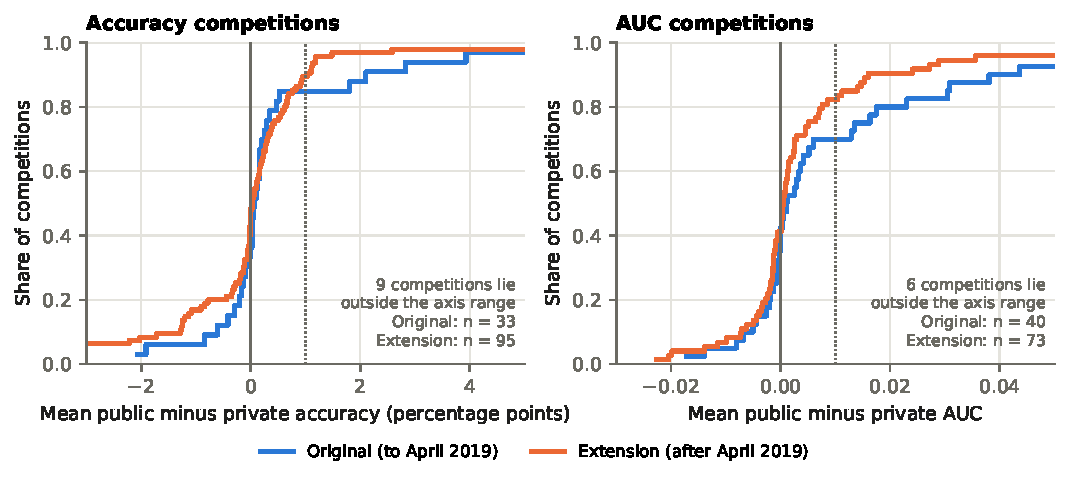
\includegraphics[width=0.9\linewidth]{figures/fig1_gap_level.pdf}
\caption{Distribution of competition mean gaps. Dotted lines mark the pre-set thresholds for a material gap.}
\label{fig:gap}
\end{figure}

\begin{figure}[t]
\centering
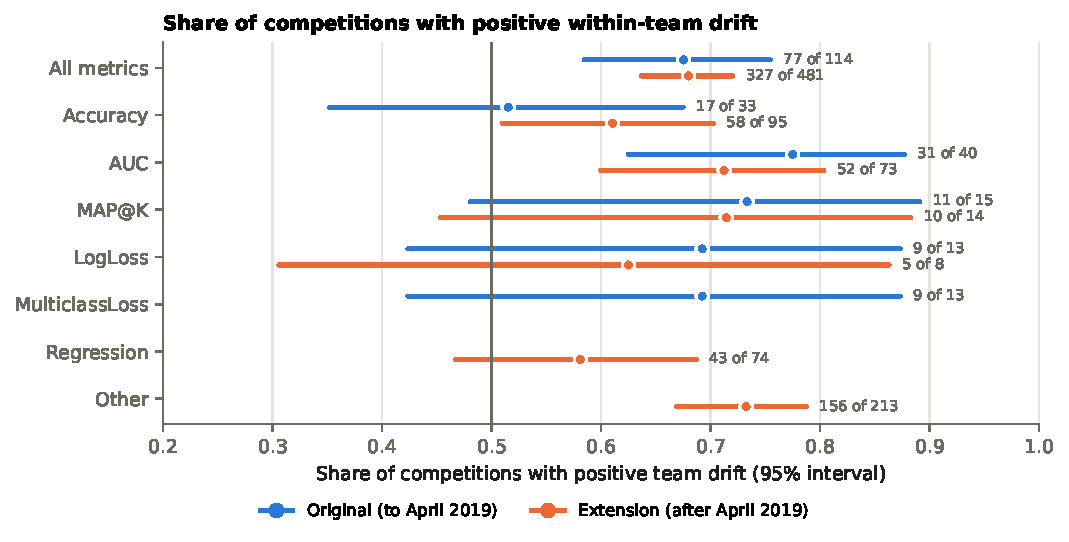
\includegraphics[width=0.9\linewidth]{figures/fig2_drift.pdf}
\caption{Share of competitions with positive within-team drift (later submissions have a larger public-over-private gap than earlier ones), by metric group, with 95\% Wilson intervals. Groups with fewer than eight competitions are omitted.}
\label{fig:drift}
\end{figure}

\section{Secondary results}

These analyses were specified in advance but are not confirmatory.

\paragraph{Regression and classification.} We find no clear difference. Median relative drift is 0.5\% for regression ($E$ and $W$, $n=124$) and 0.7\% for classification ($E$ and $O$, $n=307$); the difference is $-0.2$ points ($-1.0$, $2.1$).

\paragraph{Test-set size.} Among 125 accuracy competitions with inferred sizes, the absolute mean gap falls with total test size (Spearman $-0.61$): its median is 0.83 percentage points below 10,000 examples and 0.16 at or above (Figure~\ref{fig:size}). The top-decile gap net of the independent-resplitting reference shows no clear association with size (Spearman 0.12, $p=0.20$). Smaller test sets go with larger gaps in either direction, as sampling noise predicts. The data do not single out 10,000 as a threshold, and the lack of association for the reference-adjusted gap is not evidence of independence. Both statements depend on the minimum sizes.

\paragraph{Time and platform.} Within $E$ there is no trend in relative drift or relative gap across deadline years. Competitions scored by re-running submitted code have larger relative gaps than the rest of $E$ (median 0.30 against 0.007); Section~\ref{sec:explore} examines this.

\paragraph{Formal accuracy test.} The median share of first-per-team submissions with $p \le 0.05$ is 1.7\% in $O$ and 1.8\% in $E$; it exceeds 10\% in 9\% and 11\% of competitions. These shares are conditional on the minimum sizes: if every size were twice the minimum, the medians would be 11.1\% and 11.7\%.

\begin{figure}[t]
\centering
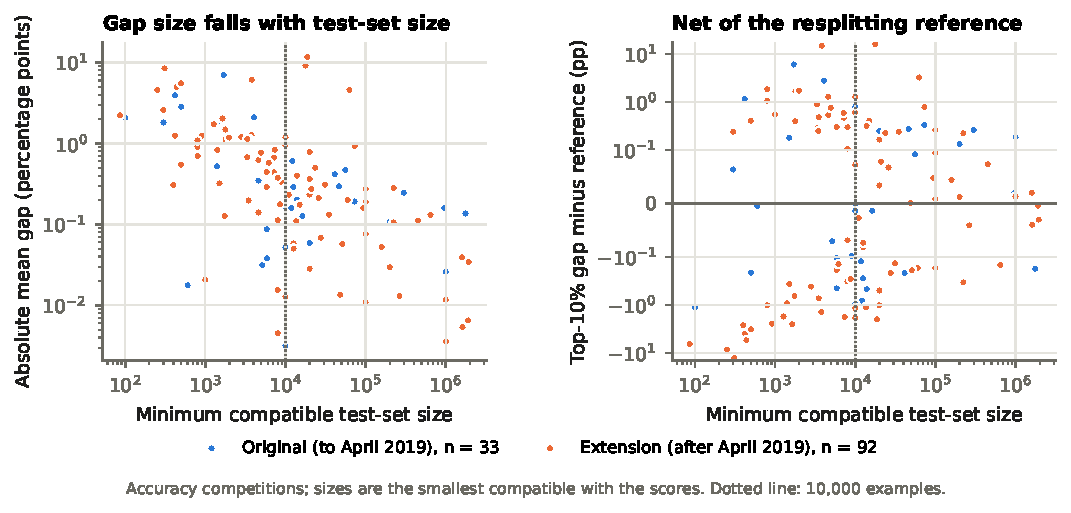
\includegraphics[width=0.9\linewidth]{figures/fig3_test_size.pdf}
\caption{Accuracy competitions: gap size, and top-decile gap net of the independent-resplitting reference, against minimum compatible test-set size.}
\label{fig:size}
\end{figure}

\section{Exploratory results}
\label{sec:explore}

The analyses in this section were chosen after the results above were known.

\paragraph{What the drift result does and does not show.} Two simple non-adaptive explanations can be set aside. Teams often begin with a trivial submission that has no gap, and gaps might scale linearly with score level; but drift is positive in 63.3\% of later competitions when only the third and fourth quarters of each team's submissions are compared, in 65.4\% after dropping each team's first two submissions, and in 66.0\% with a linear within-team control for score level. It is positive in 66.0\% of competitions whose first submissions have a negative gap. Without clipping it is positive in 63.8\% (307 of 481).

These checks do not establish adaptation. An independent review of this work constructed predetermined submission trajectories, using no feedback, in which accuracy rises along a curve and the public-minus-private difference rises linearly with position; they pass all of the checks above with a relative drift of about 1\%, including a negative first-submission gap. Such trajectories require public and private sets that differ in composition. In our simulations of feedback-free submissions whose gains differ across groups of examples, a random split gives positive drift in 45\% of 300 simulated competitions, while a split that places the fastest-improving groups in the public set gives positive drift in all of them.

The question is therefore how far splits are random, and the data say little. Only five analysed competitions state a random split (drift positive in three). Among accuracy competitions whose first submissions fit the random-split null model, drift is positive in 56 of 94 (59.6\%, $p=0.08$). First-submission gaps themselves are positive in 56\% of later competitions ($p=0.007$), which is evidence that public and private sets are not exchangeable in general, or that some adaptation precedes a team's first submission. We conclude that the divergence is real as a description and is consistent with adaptation, and that aggregate scores do not separate adaptation from model-dependent differences between the sets.

\paragraph{The original outliers.} For two of the five outliers the top-10\% gap is close to the independent-resplitting reference (difference $-0.23$ and $+0.06$ percentage points), so these gaps are compatible with selection under that reference; for the other three the gap is larger ($+6.0$, $+2.8$ and $+1.2$).

\paragraph{Featured and Research competitions.} In the Featured and Research host categories, the median relative gap is 0.17 in $E$ ($n=184$) against 0.01 in $O$ ($n=68$; $p=0.003$), and already 0.08 against 0.01 for teams' first submissions (Figure~\ref{fig:prize}). The share with positive drift is similar (72.5\% against 70.6\%). Within $E$, code-only competitions in these categories do not differ clearly from the others, so the platform contrast above is mostly one of composition. Only 23 of the 184 use one of the original five metrics, so H1 does not speak to them. Scores are also more tightly packed in recent competitions of these categories, which enlarges any gap expressed in team spreads. A gap present from the first submission is compatible with differences in how the two sets are built or scored, and also with adaptation inherited from public notebooks before a team's first submission. We have not identified the mechanism.

\begin{figure}[t]
\centering
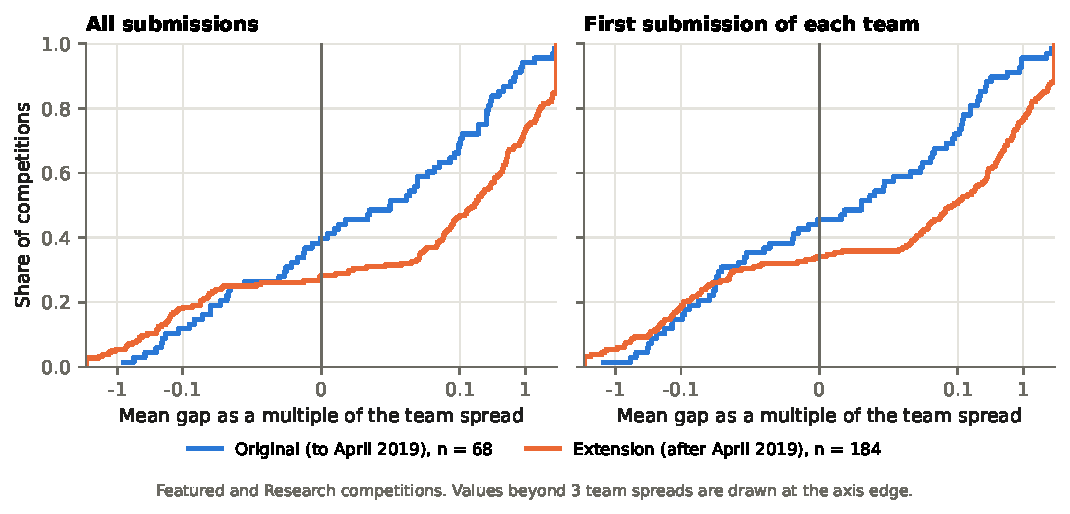
\includegraphics[width=0.9\linewidth]{figures/fig4_prize.pdf}
\caption{Featured and Research competitions: mean gap in units of the team spread, for all submissions and for teams' first submissions.}
\label{fig:prize}
\end{figure}

\section{Limitations}

Aggregate scores limit what can be identified. Drift cannot separate adaptation from model-dependent differences between non-exchangeable sets, and it cannot see adaptation that is complete before a team's first submission. Minimum compatible sizes are lower bounds; outside tiers A and B the formal test is conditional on them. The null model treats each submission as independently split, whereas all submissions share one split and are correlated, so neither the distribution of tail probabilities nor the top-decile reference has an exact interpretation. Split design is unknown for most competitions: labels record what hosts wrote, were assigned by one reader, and were checked only by that reader on excerpts.

The comparison between cohorts is by metric, not by task, host or year. Accuracy competitions are mostly in-class in both periods (25 of 33 and 82 of 95); AUC competitions are not (29 of 73 in $E$). Only two accuracy competitions in $E$ ended after 2022. Competitions are treated as independent units, although course series and recurring contests share hosts, data and participants. The study uses one snapshot of Meta Kaggle. We did not study the number of classes or notebook forking.

\section{Conclusion}

For accuracy and AUC competitions, the typical signed gap between public and private scores is as small after April 2019 as in the original sample, within margins fixed in advance. Within teams, later submissions favour the public leaderboard slightly more than earlier ones in about two thirds of competitions in both periods. That is the direction adaptation predicts, but leaderboard scores alone cannot attribute it to adaptation, because the same pattern follows from model-dependent differences between sets whose construction is mostly undocumented. Featured and Research competitions since 2019 show larger public-over-private gaps from the first submission onward, on metrics the original study did not cover. Settling these questions needs what Meta Kaggle does not contain: per-example predictions and the public--private assignment of test examples.

\subsubsection*{Reproducibility}
Code, the archived analysis plan, the label table and all result tables will be released. All scripts were re-run from the raw files in a clean environment and reproduced every table. An independent review recomputed the confirmatory tests and reproduced them exactly; its counterexample and sensitivity analyses are included with the code.

\bibliography{references}
\bibliographystyle{tmlr}
\end{document}
